\documentclass[10pt]{beamer}

\usetheme{metropolis}
\usepackage{appendixnumberbeamer}
\usepackage[croatian]{babel}
\usepackage[utf8]{inputenc}
\usepackage{graphicx}



\title{Grafička sučelja za pregled razlika i pomoć pri spajanju}
\subtitle{Seminar}
\date{\today}
\author{Paolo Licul}{Nino Dumičić}

\begin{document}

\maketitle

\begin{frame}{Sadržaj}
  \setbeamertemplate{section in toc}[sections numbered]
  \tableofcontents[hideallsubsections]
\end{frame}


\begin{frame}{Uvod}
	\begin{itemize}
		\item Grafička sučelja za pregled razlika i pomoć pri spajanju su vrlo koristan alat koji se svakodnevno koristi
		\item Temelje se na standardnim git commandama \emph{diff} i \emph{merge}
		\item Olakšavaju pregled razlika između dokumenata
		\item Za razliku od jednostavne diff komande razni alati mogu pokazati razlike i između: \begin{itemize}
		\item slika
		\item pdf i excel fileova
		\item foldera
		\end{itemize}
	\end{itemize} 
	
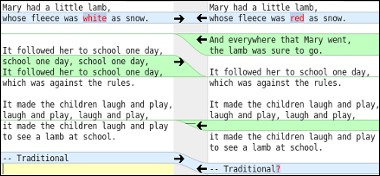
\includegraphics[width=10cm]{gui.png}
\end{frame}

\begin{frame}{WinMerge}

\includegraphics[width=2cm, height=2cm]{WinMerge1.png}
\begin{itemize}
    \item Open Source
    \item Izgledom sličan Tortoiseu
    \item Može uspoređivati i datoteke i mape
    \item Iznimna integracija s windowsom
    \item "Three way file comparison"
    \item Ukazuje na pogreške unutar linija
\end{itemize}
    
\end{frame}
\begin{frame}{Spajanje u WinMerge-u}
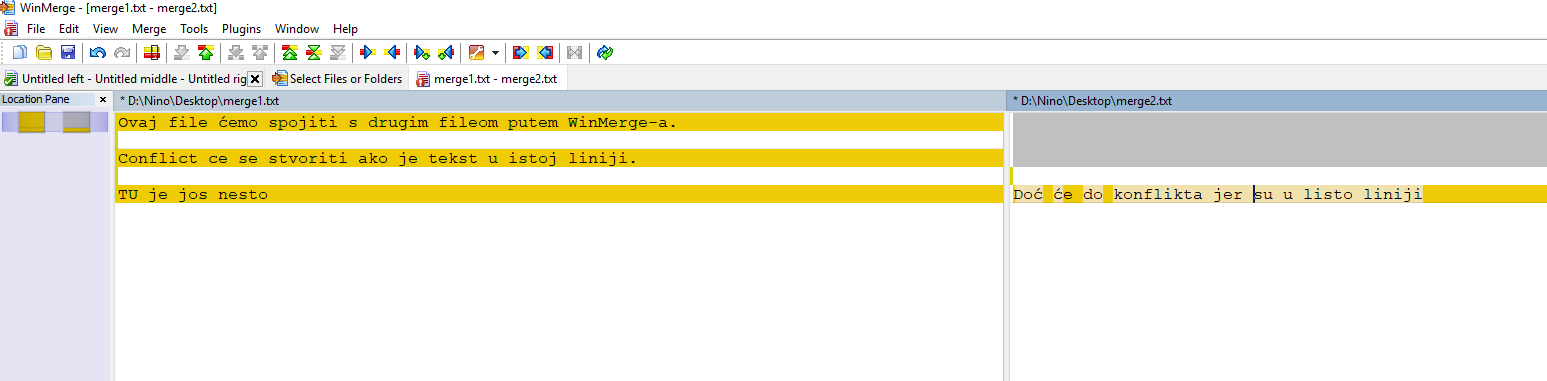
\includegraphics[width=10cm, height=5cm]{WinMerge2.png}
    
\end{frame}
\begin{frame}
    \begin{itemize}
        \item Pojavio se conflict i taj dio se neće spojiti u drugu datoteku
    \end{itemize}
    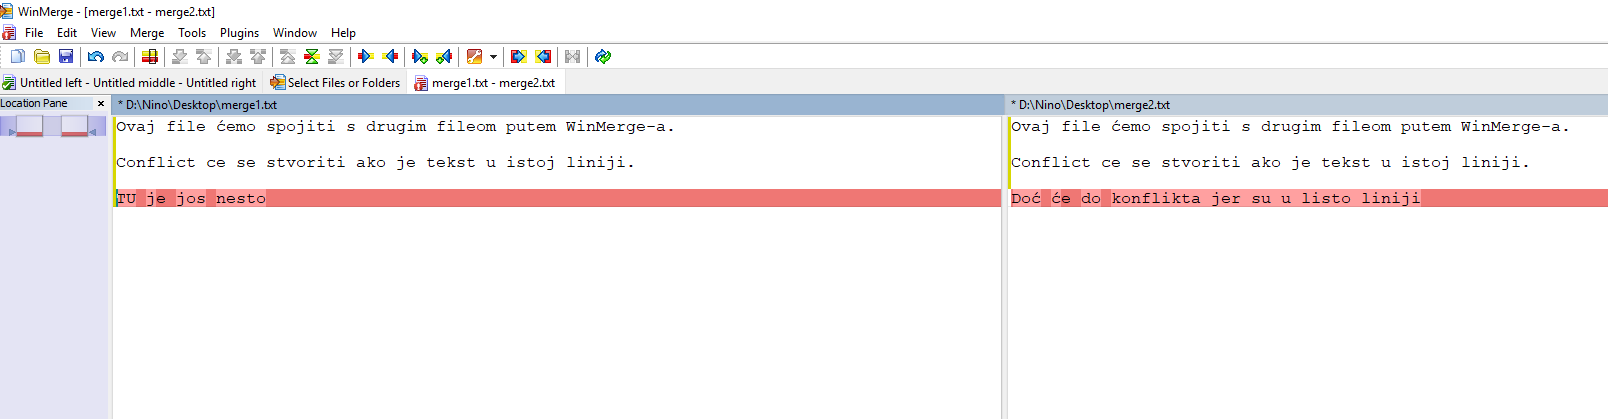
\includegraphics[width=10cm, height=5cm]{WinMerge3.png}\newline
    \begin{itemize}
        \item Prikaz datoteke nakon merge-a
    \end{itemize}
    
\includegraphics[width=5cm, height=2cm]{WinMerge4.png}
\end{frame}

\begin{frame}{Beyond compare}
	\begin{itemize}
		\item Vrlo moderan i estetski GUI
		\item Moze istovremeno raditi vise usporedba u razlicitim tabovima
		\item Moze usporedivati više tipova datoteka(slike, tablice, registare itd.)
		\item 
		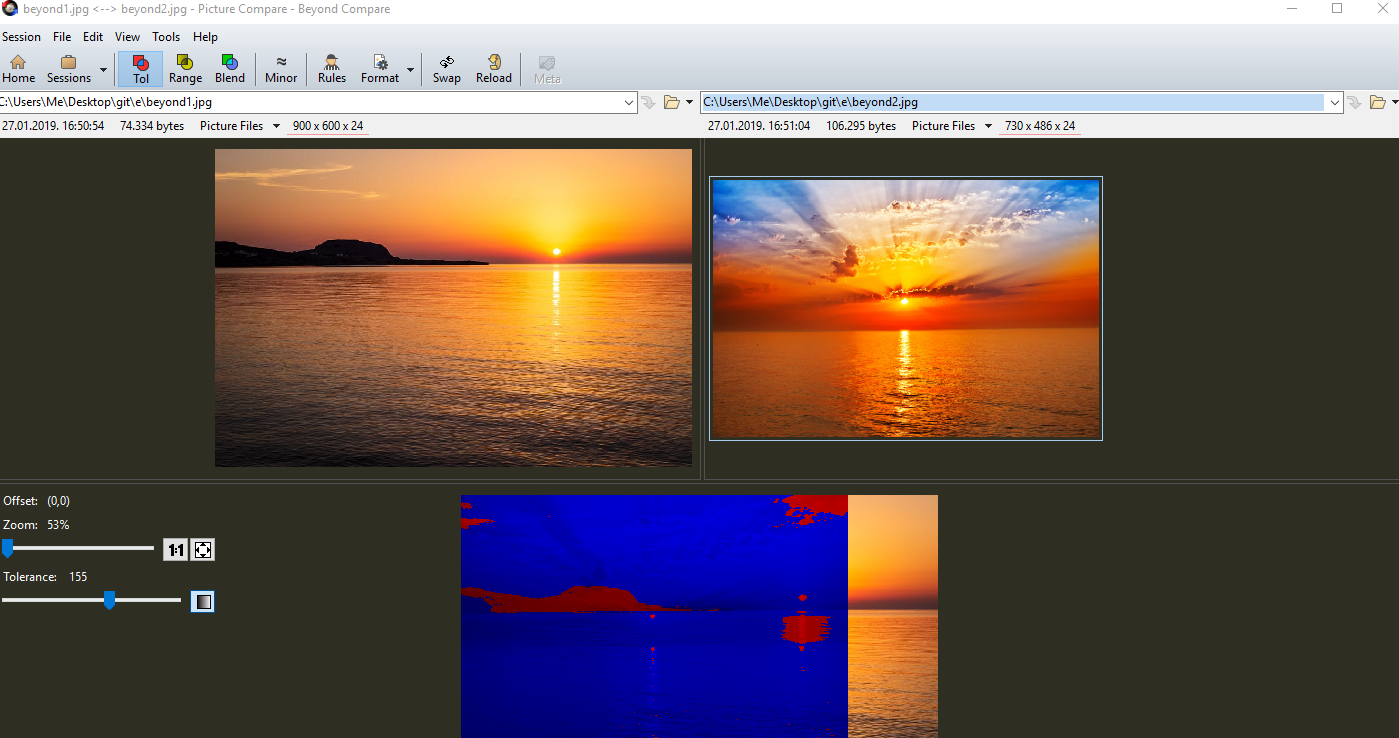
\includegraphics{beyond.png}
		\includegraphics{beyond3.png}
\end{frame}

\begin{frame}{TortoiseSVN}

\includegraphics[width=2cm, height=2cm]{tortoise4.png}
\begin{itemize}
    \item Besplatan software
    \item Open source
    \item Lagan za korištenje
    \item Jednostavno i user-friendly sučelje
    \item Graf commitova
    \item Odlično integriran s Windowsom
\end{itemize}
\end{frame}

\begin{frame}{Spajanje u Tortoiseu}
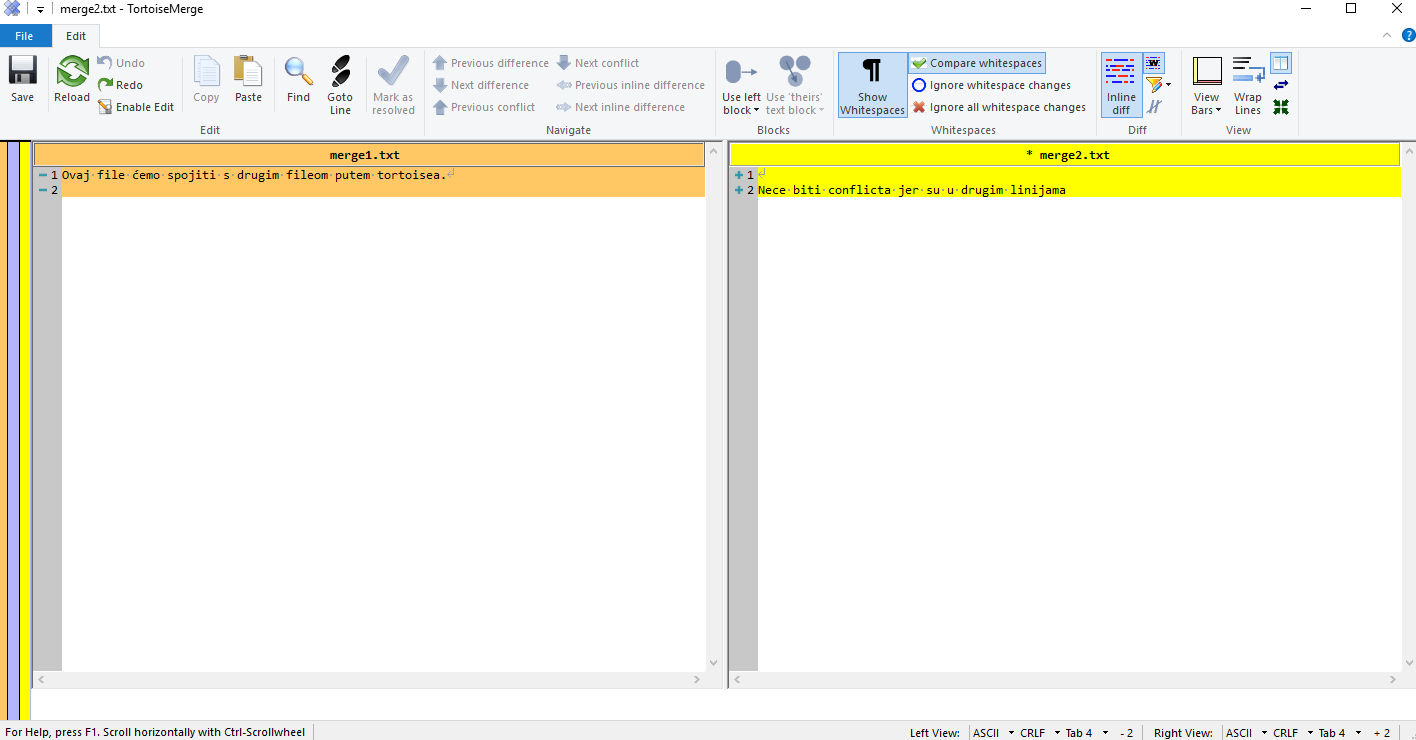
\includegraphics[width=10cm]{tortoise1.png}
\end{frame}

\begin{frame}
\begin{itemize}
    \item\small{Datoteka merge1 spojena u merge2}
\end{itemize}
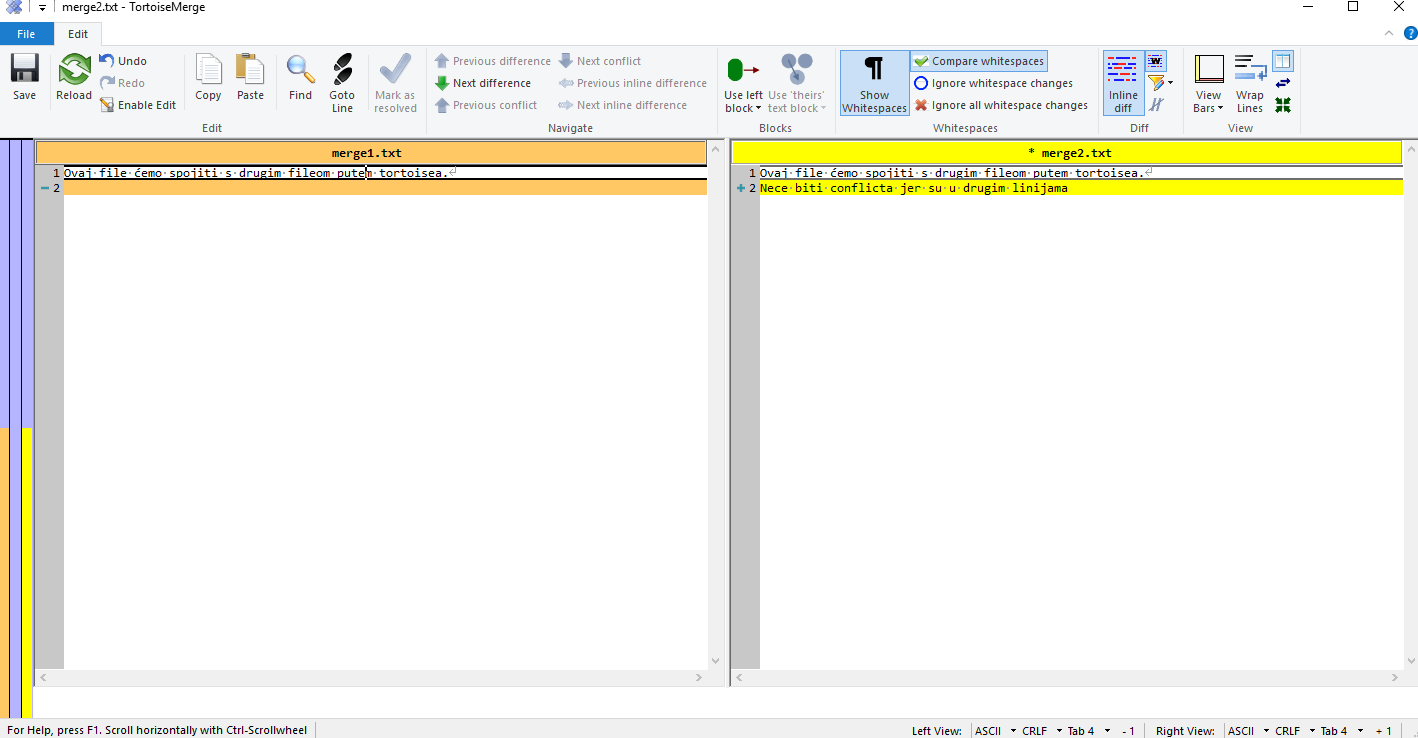
\includegraphics[height=4cm, width=10cm]{tortoise2.png}\newline
\begin{itemize}
    \item\small{Vidljivo kad otvorimo sami file}
\end{itemize}
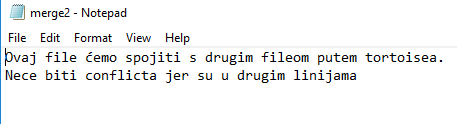
\includegraphics[width=7cm]{tortoise3.png}
\end{frame}

\begin{frame}{Kdiff 3}
	\begin{itemize}
		\item Primjer zastarjelog GUI-a 
		\item Do \emph{3} usporedbe istovremeno
		\item Moze usporedivati više tipova datoteka(slike, tablice, registare itd.)
		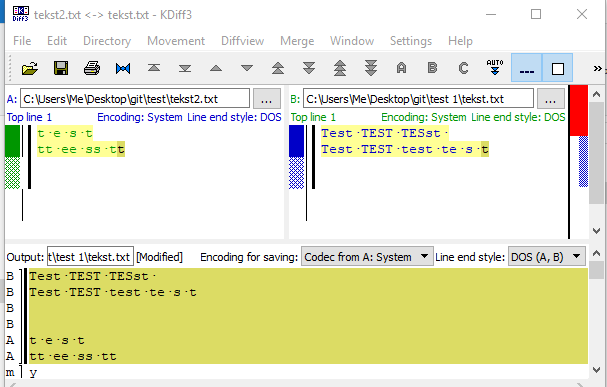
\includegraphics{kdif.png}
\end{frame}


\end{document}
